\chapter{Kruskal Algorithm with Data Structure}
\begin{algoprob}
	\problemtitle{Minimum Spanning Tree}
	\probleminput{Weighted undirected graph $G=(V,E)$ and weights of edges $W=\{w_e\in\bbZ_0\colon e\in E\}$.}
	\problemquestion{Find a spanning tree $T\subseteq E$ such that $\sum\limits_{e\in T}w_e$ is minimum.}
\end{algoprob}
In this chapter we will discuss this problem. We will first discuss the Kruskal algorithm which gives a greedy solution to the problem. Then we will discuss the data structure that we can use to implement the Kruskal algorithm efficiently.
\section{Kruskal Algorithm}
\begin{center}
	\hspace*{4mm}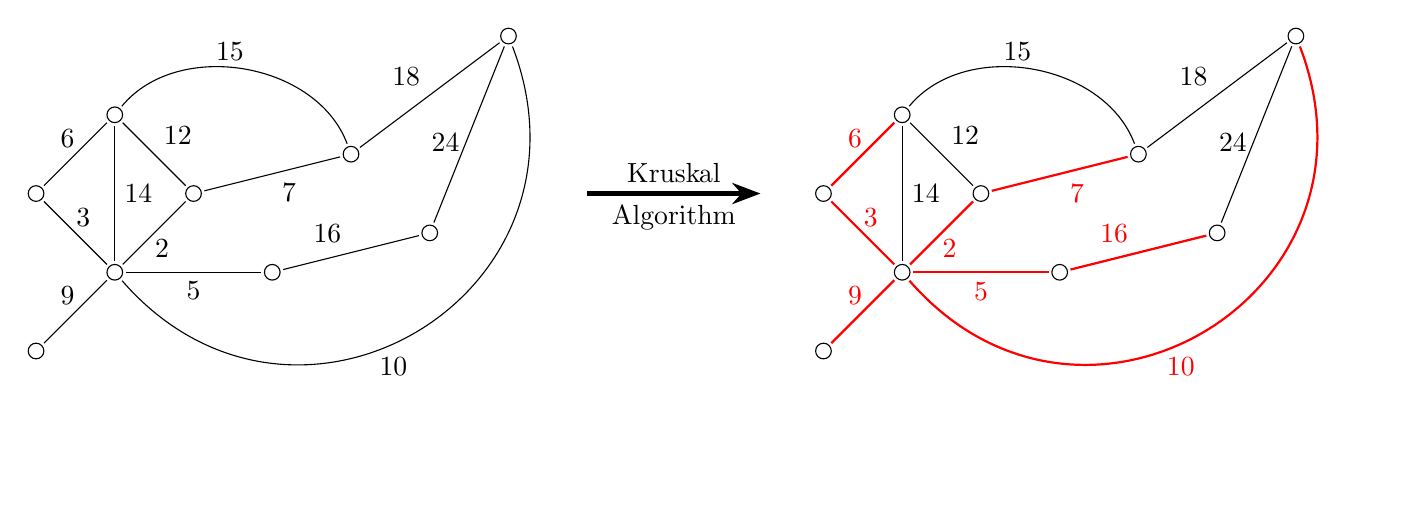
\begin{tikzpicture}[vertex/.style={circle, draw, fill=white, inner sep=2pt}]
		\begin{scope}[shift={(-5,0)}]
			\node[vertex] (1) at (0, 0) {};
			\node[vertex] (2) at (1, 1) {};
			\node[vertex] (3) at (1, -1) {};
			\node[vertex] (4) at (2, 0) {};
			\node[vertex] (5) at (4, 0.5) {};
			\node[vertex] (6) at (6, 2) {};
			\node[vertex] (7) at (5, -0.5) {};
			\node[vertex] (8) at (3, -1) {};
			\node[vertex] (9) at (0, -2) {};

			%    % Edges with weights (some edges have bends to avoid crossing)
			\draw[shorten >=1pt, shorten <=1pt] (1) -- (2) node[midway, xshift=-1mm,yshift=2mm] {6};
			\draw[shorten >=1pt, shorten <=1pt] (1) -- (3) node[midway, xshift=1mm,yshift=2mm] {3};
			\draw[shorten >=1pt, shorten <=1pt] (2) -- (3) node[midway, right] {14};
			\draw[shorten >=1pt, shorten <=1pt] (2) -- (4) node[midway, above right] {12};
			\draw[shorten >=1pt, shorten <=1pt] (3) -- (4) node[midway, xshift=1mm,yshift=-2mm] {2};
			\draw[shorten >=1pt, shorten <=1pt] (4) -- (5) node[midway, below right] {7};
			\draw[shorten >=1pt, shorten <=1pt] (2) to [bend left=60] (5) node[xshift=-1.5cm, yshift=1.2cm] {15};
			\draw[shorten >=1pt, shorten <=1pt] (5) -- (6) node[midway, above left] {18};
			\draw[shorten >=1pt, shorten <=1pt] (6) -- (7) node[midway, xshift=-3mm, yshift=-1mm] {24};
			\draw[shorten >=1pt, shorten <=1pt] (7) -- (8) node[midway, above left]{16};
			\draw[shorten >=1pt, shorten <=1pt] (3) -- (8) node[midway, below] {5};
			\draw[shorten >=1pt, shorten <=1pt] (3) to [bend right=80, looseness=1.5] (6) node[xshift=-1.5cm, yshift=-4.1cm] {10};
			\draw[shorten >=1pt, shorten <=1pt] (3) -- (9) node[midway, xshift=-1mm,yshift=2mm] {9};
		\end{scope}
		\draw[ultra thick, -Stealth] (2,0)  -- (4.2,0) node[midway, above] {Kruskal} node[midway, below] {Algorithm};
		\begin{scope}[shift={(5,0)}]
			\node[vertex] (1) at (0, 0) {};
			\node[vertex] (2) at (1, 1) {};
			\node[vertex] (3) at (1, -1) {};
			\node[vertex] (4) at (2, 0) {};
			\node[vertex] (5) at (4, 0.5) {};
			\node[vertex] (6) at (6, 2) {};
			\node[vertex] (7) at (5, -0.5) {};
			\node[vertex] (8) at (3, -1) {};
			\node[vertex] (9) at (0, -2) {};

			%    % Edges with weights (some edges have bends to avoid crossing)
			\draw[shorten >=1pt, shorten <=1pt, red, thick] (1) -- (2) node[midway, xshift=-1mm,yshift=2mm] {6};
			\draw[shorten >=1pt, shorten <=1pt, red, thick] (1) -- (3) node[midway, xshift=1mm,yshift=2mm] {3};
			\draw[shorten >=1pt, shorten <=1pt] (2) -- (3) node[midway, right] {14};
			\draw[shorten >=1pt, shorten <=1pt] (2) -- (4) node[midway, above right] {12};
			\draw[shorten >=1pt, shorten <=1pt, red, thick] (3) -- (4) node[midway, xshift=1mm,yshift=-2mm] {2};
			\draw[shorten >=1pt, shorten <=1pt, red, thick] (4) -- (5) node[midway, below right] {7};
			\draw[shorten >=1pt, shorten <=1pt] (2) to [bend left=60] (5) node[xshift=-1.5cm, yshift=1.2cm] {15};
			\draw[shorten >=1pt, shorten <=1pt] (5) -- (6) node[midway, above left] {18};
			\draw[shorten >=1pt, shorten <=1pt] (6) -- (7) node[midway, xshift=-3mm, yshift=-1mm] {24};
			\draw[shorten >=1pt, shorten <=1pt, red, thick] (7) -- (8) node[midway, above left]{16};
			\draw[shorten >=1pt, shorten <=1pt, red, thick] (3) -- (8) node[midway, below] {5};
			\draw[shorten >=1pt, shorten <=1pt, red, thick] (3) to [bend right=80, looseness=1.5] (6) node[xshift=-1.5cm, yshift=-4.1cm] {10};
			\draw[shorten >=1pt, shorten <=1pt, red, thick] (3) -- (9) node[midway, xshift=-1mm,yshift=2mm] {9};
		\end{scope}
	\end{tikzpicture}
\end{center}
The Kruskal algorithm uses a concept of component to find the minimum spanning tree.
\begin{Definition}{Component}{}
	In a graph $G=(V,E)$, a \emph{component} is a maximal subgraph $G'=(V',E')$ of $G$ such that \begin{enumerate}[label=(\arabic*)]
		\item $(V',E')$ is connected.
		\item $\forall\ v\notin V'$, there is no edge $e\in E$ such that $e$ connects $v$ to any vertex in $V'$.
	\end{enumerate}
\end{Definition}
In Kruskal algorithm we maintain a set of components each of them is a tree so basically we maintain a forest. And we find a safe edge which is always the least weight edge in the graph that connects two distinct components and add that edge to the collection of edges in the forest and update the components.

So the algorithm first sorts the edges in non-decreasing order of their weights. Then it initializes a forest $F$ with all the vertices in the graph and no edges. Then it iterates through the sorted edges and checks if the edge connects two distinct components. If it does, then it adds the edge to the forest and merges the two components. The algorithm stops when we have $n-1$ edges in the forest.
\begin{algorithm}[]
	\SetKwComment{Comment}{// }{}
	\caption{\textsc{Kruskal Algorithm}}
	\DontPrintSemicolon
	\KwIn{$G=(V,E)$, and weights of edges $W=\{w_e\in\bbZ_0\colon e\in E\}$}
	\KwOut{A minimum spanning tree $T\subseteq E$ of $G$}
	\Begin{
		\If{$G$ is not connected}{
			\Return{None}\Comment*{Use DFS or BFS}
		}
		$T\longleftarrow\emptyset$\;
		Sort the edges in $E$ in non-decreasing order of their weights so that $w(e_1)\leq w(e_2)\leq\cdots \leq w(e_m)$\;
		\For{$i=1,\dots, m$}{
			Let $e_i=(u,v)$\;
			\If{$T\cup\{e_i\}$ is acyclic}{
				$T\longleftarrow T\cup\{e_i\}$
			}
			\If{$|T|=|V|-1$}{
				\Return{$T$}\;
			}
		}
	}
\end{algorithm}
We have shown in \lmref{graphic-matroid} that the set of collection of acyclic sets in any graph is a matroid. Hence, here we are basically finding a base of the graphic matroid with minimum weight. The algorithm is exactly similar to the greedy algorithm for finding max-weight base of a matroid in \autoref{matroid-max-weight-base}. So you can use the similar arguments to show that the algorithm is correct and returns the minimum spanning tree of the graph.

Now in the algorithm the checking of $T\cup \{e_i\}$ is acyclic can be done by checking if both the end points are in same component or not. And if they are not then we need to combine those to components. But there comes a question:
\begin{question}{}
	What it means to give a component?
\end{question}
We will use some vertex to represent the component. We keep a pointer $v.\emph{parent}$ for each vertex which points to representative of component $v$ is in. Hence, we need a data structure that can do the following two operations efficiently:
\begin{itemize}[label=$\bullet$]
	\item \textsc{Find}$(u)$: Returns the component $u$ is in.
	\item \textsc{Union}$(u,v)$: Merges the components of $u$ and $v$ into a single component.
\end{itemize}
So we can use the updated algorithm to implement the Kruskal algorithm  using proper data structure:
\begin{algorithm}[]
	\SetKwComment{Comment}{// }{}
	\caption{\textsc{Kruskal Algorithm}}
	\DontPrintSemicolon
	\KwIn{$G=(V,E)$, and weights of edges $W=\{w_e\in\bbZ_0\colon e\in E\}$}
	\KwOut{A minimum spanning tree $T\subseteq E$ of $G$}
	\Begin{
		\If{$G$ is not connected}{
			\Return{None}\Comment*{Use DFS or BFS}
		}
		$T\longleftarrow\emptyset$\;
		Sort the edges in $E$ in non-decreasing order of their weights so that $w(e_1)\leq w(e_2)\leq\cdots \leq w(e_m)$\;
		\For{$i=1,\dots, m$}{
			Let $e_i=(u,v)$\;
			\If{$\textsc{Find}(u)\neq \textsc{Find}(v)$}{
				$T\longleftarrow T\cup\{e_i\}$\;
				\textsc{Union}$(u,v)$
			}
			\If{$|T|=|V|-1$}{
				\Return{$T$}\;
			}
		}
	}
\end{algorithm}
The Kruskal Algorithm calls $m$ times the \textsc{Find} operation and $n$ times the \textsc{Union} operation.
\section{Data Structure 1: Linear Array}
We create an $n$ length array $A$ which hold the parent pointer of each vertex. Initially for all vertices $A[v]=v$. So \textsc{Array-Find}$(u)$ will just return $A[u]$. Hence \textsc{Find} takes $O(1)$ time. For \textsc{Union}$(u,v)$ we use the following:
\begin{algorithm}[]
	\caption{\textsc{Array-Union}$(u,v)$}
	\DontPrintSemicolon
	\If{$A[u]\neq A[v]$}{
	\For{$i=1,\dots, n$}{
	\If{ $A[i]==A[v]$}{
	$A[i]\longleftarrow A[u]$\;
	}
	}
	}
\end{algorithm}
Therefore, \textsc{Array-Union}$(u,v)$ takes $O(n)$ time. Hence, the time complexity of the Kruskal algorithm using this data structure is $m\cdot O(1)+n\cdot O(n)=O(m+n^2)=O(n^2)$.
\section{Data Structure 2: Left Child Right Siblings Tree}
Using an array is not efficient enough.  One place we can optimize is if given the components is there a faster way to get the vertices in the component?  We can use the following tricks to optimize:
\begin{enumerate}[]
	\item For every representative of a component, store pointers to all vertices in that component.
	\item Change representative for the smaller component while doing \textsc{Union}$(u,v)$.
\end{enumerate}
\subsection{Construction}
So now every representative of a component we point to one vertex which is also in the component. And from that vertex we can iterate through all the vertices in that component. So basically we can immagine a 2 level tree where all the children point towards the root which is the representative of the component. The root points to one of the children take the left most child. And then all the other children points to the immediate right child of the root.
\begin{center}
	\usetikzlibrary{arrows.meta}
	\begin{tikzpicture}[vertex/.style={circle, draw, fill=white, inner sep=2pt}]
		\begin{scope}
			\node at (-2,0) {Initially we had:};
			\node[vertex] (1) at (0, 0) {};
			\node[vertex] (21) at (1, 0) {};
			\node[vertex] (22) at (1, -1) {};
			\node[vertex] (31) at (3, 0) {};
			\node[vertex] (32) at (2, -1) {};
			\node[vertex] (33) at (3, -1) {};
			\node[vertex] (34) at (4, -1) {};
			\node[vertex] (41) at (5, 0) {};
			\node[vertex] (42) at (5, -1) {};
			\path (1) edge [out=120, in=60, loop, min distance=0.4cm, -{Latex[length=1mm]}] (1);
			\path (21) edge [out=120, in=60, loop, min distance=0.4cm, -{Latex[length=1mm]}] (21);
			\path (31) edge [out=120, in=60, loop, min distance=0.4cm, -{Latex[length=1mm]}] (31);
			\path (41) edge [out=120, in=60, loop, min distance=0.4cm, -{Latex[length=1mm]}] (41);
			\draw[-{Latex[length=1mm]}] (22) -- (21);
			\draw[-{Latex[length=1mm]}] (42) -- (41);
			\foreach \x in {2,3,4} {
			\draw[-{Latex[length=1mm]}] (3\x) -- (31);
			}
			\path (31) edge[bend right=30, -{Latex[length=1mm]}, red] node[midway, left, font=\tiny] {Want} (32);
			\path (32) edge[-{Latex[length=1mm]}, red] node[midway, below, font=\tiny] {Want} (33);
		\end{scope}
		\begin{scope}[shift={(0,-2)}]
			\node at (-2,0) {Now we will do:};
			\node[vertex] (1) at (0, 0) {};
			\node[vertex] (21) at (1, 0) {};
			\node[vertex] (22) at (1, -1) {};
			\node[vertex] (31) at (3, 0) {};
			\node[vertex] (32) at (2, -1) {};
			\node[vertex] (33) at (3, -1) {};
			\node[vertex] (34) at (4, -1) {};
			\node[vertex] (41) at (5, 0) {};
			\node[vertex] (42) at (5, -1) {};
			\path (1) edge [out=120, in=60, loop, min distance=0.4cm, -{Latex[length=1mm]}] (1);
			\path (21) edge [out=120, in=60, loop, min distance=0.4cm, -{Latex[length=1mm]}] (21);
			\path (31) edge [out=120, in=60, loop, min distance=0.4cm, -{Latex[length=1mm]}] (31);
			\path (41) edge [out=120, in=60, loop, min distance=0.4cm, -{Latex[length=1mm]}] (41);
			\foreach \x in {2,4} {
					\draw[-right to,shorten <=1.15mm, shorten >=1.15mm] ($(\x2)+(0.02,0)$) -- ($(\x1)+(0.02,0)$);
					\draw[-right to,shorten <=1.15mm, shorten >=1.15mm] ($(\x1)+(-0.02,0)$) -- ($(\x2)+(-0.02,0)$);
				}
			\foreach \x in {3,4} {
			\draw[-{Latex[length=1mm]}] (3\x) -- (31);
			}
			\draw[-right to,shorten <=1mm, shorten >=1.2mm] ($(32)+(0.03,0)$) -- ($(31)+(0.03,0)$);
			\draw[-right to,shorten <=1mm, shorten >=1.2mm] ($(31)+(-0.03,0)$) -- ($(32)+(-0.03,0)$);
			\draw[-{Latex[length=1mm]}] (32) -- (33);
			\draw[-{Latex[length=1mm]}] (33) -- (34);
		\end{scope}
	\end{tikzpicture}
	\captionof{figure}{Left Child Right Sibling}
\end{center}
We can also store a variable to store the number of vertices in the component so that we can use it to compare the size of two components and then update for the smaller one. Therefore, the data structure now stores:
\begin{itemize}
	\item $v.\emph{parent}$ for each $v$ which points to the vertex representing the component $v$ is in.
	\item $v.\emph{size}$ for size of the component for each component representative $v$.
	\item $v.\emph{left}$ for the left most child for each component representative $v$.
	\item $v.\emph{right}$ for the immediate right sibling of $v$ for all vertices in a component which are not  representatives of the components.
\end{itemize}\parinf

This data structure is called Left Child Right Sibling. So in this data structure the \textsc{LCRS-Find}$(u)$ just returns the value of $u.\emph{parent}$. Hence, \textsc{LCRS-Find} takes $O(1)$ time.
\subsection{\textsc{LCRS-Union} Function}
For the \textsc{LCRS-Union} function we do the following
\begin{algorithm}[]
	\caption{\textsc{LCRS-Union}$(u,v)$}
	\DontPrintSemicolon
	$up\longleftarrow u.\emph{parent}$\; $vp\longleftarrow v.\emph{parent}$\;
	\If{$up\neq vp$}{
		\If{$up==u$}{
			$u.\emph{parent}\longleftarrow vp$\; $u.\emph{right}\longleftarrow vp.\emph{left}$\;
			$vp.\emph{left}\longleftarrow u$\; $vp.\emph{size}\longleftarrow vp.\emph{size}+1$\;
		}
		\ElseIf{$up.\emph{size}\leq vp.\emph{size}$}{
			$up.\emph{right}\longleftarrow u$\;
			$x\longleftarrow up$\;
			\While{$x.\emph{right}==None$}{
				$x.\emph{parent}\longleftarrow vp$, $x\longleftarrow x.\emph{right}$
			}
			$x.\emph{right}\longleftarrow vp.\emph{left}$\;
			$vp.\emph{left}\longleftarrow up.\emph{left}$\;
			$vp.\emph{left}\longleftarrow up$\;
			$vp.\emph{size}\longleftarrow vp.\emph{size}+\emph{up}.size$\;
		}
		\Else{
			$vp.\emph{right}\longleftarrow v$\;
			$x\longleftarrow vp$\;
			\While{$x.\emph{right}==None$}{
				$x.\emph{parent}\longleftarrow up$, $x\longleftarrow x.\emph{right}$
			}
			$x.\emph{right}\longleftarrow up.\emph{left}$\;
			$up.\emph{left}\longleftarrow vp.\emph{left}$\;
			$up.\emph{left}\longleftarrow vp$\;
			$up.\emph{size}\longleftarrow up.\emph{size}+\emph{vp}.size$\;
		}
	}
\end{algorithm}

Below we have shown how the \textsc{LCRS-Union} function works.
\begin{figure}[!h]
	\centering
	\begin{tikzpicture}[vertex/.style={circle, draw, fill=white, inner sep=2pt}]
		\begin{scope}
			\node at (-1,0) {(a)};
			\node[vertex] (21) at (0, 0) {};
			\node[vertex] (22) at (0, -1) {};
			\node[vertex] (31) at (2, 0) {};
			\node[vertex] (32) at (1, -1) {};
			\node[vertex] (33) at (2, -1) {};
			\node[vertex] (34) at (3, -1) {};
			\node[xshift=-0.3cm] at (0,0) {$up$};
			\node[xshift=0.3cm] at (2,0) {$vp$};
			\path (21) edge [out=120, in=60, loop, min distance=0.4cm, -{Latex[length=1mm]}] (21);
			\path (31) edge [out=120, in=60, loop, min distance=0.4cm, -{Latex[length=1mm]}] (31);
			\draw[-right to,shorten <=1.15mm, shorten >=1.15mm] ($(22)+(0.02,0)$) -- ($(21)+(0.02,0)$);
			\draw[-right to,shorten <=1.15mm, shorten >=1.15mm] ($(21)+(-0.02,0)$) -- ($(22)+(-0.02,0)$);
			\foreach \x in {3,4} {
			\draw[-{Latex[length=1mm]}] (3\x) -- (31);
			}
			\draw[-right to,shorten <=1mm, shorten >=1.2mm] ($(32)+(0.03,0)$) -- ($(31)+(0.03,0)$);
			\draw[-right to,shorten <=1mm, shorten >=1.2mm] ($(31)+(-0.03,0)$) -- ($(32)+(-0.03,0)$);
			\draw[-{Latex[length=1mm]}] (32) -- (33)  node[below]{$v$};
			\draw[-{Latex[length=1mm]}] (33) -- (34);
			\node at (22) [below] {$u$};
		\end{scope}
		\begin{scope}[shift={(5,0)}]
			\node at (0,0) {(b)};
			\node[vertex] (21) at (0, -1) {};
			\node[vertex] (22) at (1, -1) {};
			\node[vertex] (31) at (3, 0) {};
			\node[vertex] (32) at (2, -1) {};
			\node[vertex] (33) at (3, -1) {};
			\node[vertex] (34) at (4, -1) {};
			\node[below] at (0, -1) {$up$};
			\node[xshift=0.3cm] at (3,0) {$vp$};
			\draw[-{Latex[length=1mm]}] (22) -- (21);
			\path (21) edge[bend right=30, red, -{Latex[length=1mm]}] node [midway, below, font=\tiny, yshift=0.05cm]{\emph{right}} (22);
			\path (21) edge [out=120, in=60, loop, min distance=0.4cm, -{Latex[length=1mm]}] (21);
			\path (31) edge [out=120, in=60, loop, min distance=0.4cm, -{Latex[length=1mm]}] (31);
			\foreach \x in {3,4} {
			\draw[-{Latex[length=1mm]}] (3\x) -- (31);
			}
			\draw[-right to,shorten <=1mm, shorten >=1.2mm] ($(32)+(0.03,0)$) -- ($(31)+(0.03,0)$);
			\draw[-right to,shorten <=1mm, shorten >=1.2mm] ($(31)+(-0.03,0)$) -- ($(32)+(-0.03,0)$);
			\draw[-{Latex[length=1mm]}] (32) -- (33)  node[below]{$v$};
			\draw[-{Latex[length=1mm]}] (33) -- (34);
			\node at (22) [below] {$u$};
		\end{scope}
		\begin{scope}[shift={(11,0)}]
			\node at (0,0) {(c)};
			\node[vertex] (21) at (0, -1) {};
			\node[vertex] (22) at (1, -1) {};
			\node[vertex] (31) at (3, 0) {};
			\node[vertex] (32) at (2, -1) {};
			\node[vertex] (33) at (3, -1) {};
			\node[vertex] (34) at (4, -1) {};
			\node[below] at (0, -1) {$up$};
			\node[xshift=0.3cm] at (3,0) {$vp$};
			\path (21) edge[-{Latex[length=1mm]}] node [midway, below, font=\tiny, yshift=0.05cm]{\emph{right}} (22);
			\path (21) edge [bend left=15, -{Latex[length=1mm]}, red] node [midway, above, font=\tiny, rotate=13,yshift=-0.05cm] {\emph{parent}} (31);
			\path (22) edge [-{Latex[length=1mm]}, red] node [midway, above, font=\tiny, rotate=22, xshift=-0.3cm, yshift=-0.09cm] {\emph{parent}} (31);
			\path (31) edge [out=120, in=60, loop, min distance=0.4cm, -{Latex[length=1mm]}] (31);
			\draw[-{Latex[length=1mm]}] (21) -- (22);
			\foreach \x in {3,4} {
			\draw[-{Latex[length=1mm]}] (3\x) -- (31);
			}
			\draw[-right to,shorten <=1mm, shorten >=1.2mm] ($(32)+(0.03,0)$) -- ($(31)+(0.03,0)$);
			\draw[-right to,shorten <=1mm, shorten >=1.2mm] ($(31)+(-0.03,0)$) -- ($(32)+(-0.03,0)$);
			\draw[-{Latex[length=1mm]}] (32) -- (33)  node[below]{$v$};
			\draw[-{Latex[length=1mm]}] (33) -- (34);
			\node at (22) [below] {$u$};
		\end{scope}
		\begin{scope}[shift={(-1,-3)}]
			\node at (0,0) {(d)};
			\node[vertex] (21) at (0, -1) {};
			\node[vertex] (22) at (1, -1) {};
			\node[vertex] (31) at (3, 0) {};
			\node[vertex] (32) at (2, -1) {};
			\node[vertex] (33) at (3, -1) {};
			\node[vertex] (34) at (4, -1) {};
			\node[below] at (0, -1) {$up$};
			\node[xshift=0.3cm] at (3,0) {$vp$};
			\path (21) edge[-{Latex[length=1mm]}] node [midway, below, font=\tiny, yshift=0.05cm]{\emph{right}} (22);
			\path (21) edge [bend left=15, -{Latex[length=1mm]}] node [midway, above, font=\tiny, rotate=13,yshift=-0.05cm] {\emph{parent}} (31);
			\path (22) edge [-{Latex[length=1mm]}] node [midway, above, font=\tiny, rotate=22, xshift=-0.3cm, yshift=-0.09cm] {\emph{parent}} (31);
			\draw[-{Latex[length=1mm]},red] (22) -- node [midway, below, font=\tiny, yshift=0.05cm]{\emph{right}} (32);
			\path (31) edge [out=120, in=60, loop, min distance=0.4cm, -{Latex[length=1mm]}] (31);
			\draw[-{Latex[length=1mm]}] (21) -- (22);
			\foreach \x in {3,4} {
			\draw[-{Latex[length=1mm]}] (3\x) -- (31);
			}
			\draw[-right to,shorten <=1mm, shorten >=1.2mm] ($(32)+(0.03,0)$) -- ($(31)+(0.03,0)$);
			\draw[-right to,shorten <=1mm, shorten >=1.2mm] ($(31)+(-0.03,0)$) -- ($(32)+(-0.03,0)$);
			\draw[-{Latex[length=1mm]}] (32) -- (33)  node[below]{$v$};
			\draw[-{Latex[length=1mm]}] (33) -- (34);
			\node at (22) [below] {$u$};
		\end{scope}
		\begin{scope}[shift={(5,-3)}]
			\node at (0,0) {(e)};
			\node[vertex] (21) at (0, -1) {};
			\node[vertex] (22) at (1, -1) {};
			\node[vertex] (31) at (3, 0) {};
			\node[vertex] (32) at (2, -1) {};
			\node[vertex] (33) at (3, -1) {};
			\node[vertex] (34) at (4, -1) {};
			\node[below] at (0, -1) {$up$};
			\node[xshift=0.3cm] at (3,0) {$vp$};
			\path (21) edge[-{Latex[length=1mm]}]  (22);
			\path (22) edge [-{Latex[length=1mm]}]  (31);
			\draw[-{Latex[length=1mm]}] (22) --  (32);
			\path (31) edge [out=120, in=60, loop, min distance=0.4cm, -{Latex[length=1mm]}] (31);
			\draw[-{Latex[length=1mm]}] (21) -- (22);
			\foreach \x in {3,4} {
			\draw[-{Latex[length=1mm]}] (3\x) -- (31);
			}
			\draw[-{Latex[length=1mm]}] (32) -- (31);
			\draw[-{Latex[length=1mm]}] (32) -- (33)  node[below]{$v$};
			\draw[-{Latex[length=1mm]}] (33) -- (34);
			\draw[-{Latex[length=1mm]}] (21) -- (31);
			\node at (22) [below] {$u$};
			\path (31) edge [bend right=15, -{Latex[length=1mm]}, red] node [midway, above, font=\tiny, rotate=13,yshift=-0.05cm] {\emph{left}} (21);
		\end{scope}
		\begin{scope}[shift={(11,-3)}]
			\node at (0,0) {(f)};
			\node[vertex] (21) at (0, -1) {};
			\node[vertex] (22) at (1, -1) {};
			\node[vertex] (31) at (3, 0) {};
			\node[vertex] (32) at (2, -1) {};
			\node[vertex] (33) at (3, -1) {};
			\node[vertex] (34) at (4, -1) {};
			\path (21) edge[-{Latex[length=1mm]}]  (22);
			\path (22) edge [-{Latex[length=1mm]}]  (31);
			\draw[-{Latex[length=1mm]}] (22) --  (32);
			\path (31) edge [out=120, in=60, loop, min distance=0.4cm, -{Latex[length=1mm]}] (31);
			\draw[-{Latex[length=1mm]}] (21) -- (22);
			\foreach \x in {3,4} {
			\draw[-{Latex[length=1mm]}] (3\x) -- (31);
			}
			\draw[-{Latex[length=1mm]}] (32) -- (31);
			\draw[-{Latex[length=1mm]}] (32) -- (33)  node[below]{$v$};
			\draw[-{Latex[length=1mm]}] (33) -- (34);
			\node at (22) [below] {$u$};
			\draw[-right to,shorten <=1 mm, shorten >=1.5mm] ($(21)+(0.03,0.02)$) -- ($(31)+(0.03,0.02)$);
			\draw[-right to,shorten <=1mm, shorten >=1.2mm] ($(31)+(-0.03,0.05)$) -- ($(21)+(-0.03,0.05)$);
		\end{scope}
	\end{tikzpicture}
	\caption{A run of \textsc{LCRS-Union}$(u,v)$}
\end{figure}
This way we can unite two components and update the corresponding component representative in the vertices of the smaller component. In the next section we will analyze the amortized time complexity of the \textsc{LCRS-Union} function
\subsection{Amortized analysis of \textsc{LCRS-Union}}
\begin{lemma}{}{}
	For any vertex $v\in V$, $v.\emph{parent}$ can change at most $O(\log n)$ times.
\end{lemma}
\begin{proof}
	Initially size of $v$'s component is $1$. Each time $v.\emph{parent}$ is changed the size of the component $v$ is in becomes at least double. Therefore, at most $O(\log n)$ times $v.\emph{parent}$ can change.
\end{proof}\parinn

Now since there are $n$ vertices at most $O(n\log n)$ times change of \emph{parent} for any vertex happens. Now change of \emph{parent} for any vertex happens only in \textsc{LCRS-Union} function. Total time taken by all the \textsc{LCRS-Union} operations is $O(n\log n)$ time. Since \textsc{LCRS-Union} was called $n$ times the amortized cost of \textsc{LCRS-Union} is $O(\log n)$.
\subsection{Time Complexity Analysis of Kruskal}
We have shown above that \textsc{LCRS-Find} takes $O(1)$ time and amortized cost of \textsc{LCRS-Union} is $O(\log n)$. Since \textsc{LCRS-Find} is called $m$ times and \textsc{LCRS-Union} is called $n$ times the total run time of Kruskal Algorithm using the Left Child Right Sibling data structure is $O(m+n\log n)$.
\section{Data Structure 3: Union Find}
We will now give up on the idea of height $1$ trees to optimize more. Representative of a component is still vertex at root, but we will do the following: changes:
\begin{itemize}
	\item \textsc{Union} just changes parent pointers of root nodes, but it takes $O(1)$.
	\item Instead of size, we will maintain a variable \emph{rank} of a component roughly which can be thought of as height of the component.
	\item For \textsc{Union} root of smaller rank will be changed to point to root of the component of larger rank.
	\item The \textsc{Find} operation does something called path compression which we will explain later.
\end{itemize}
To implement this data structure we will use a tree for each component and every node has a \emph{parent} pointer. And there we will use the \textsc{Find} and \textsc{Union} operations.

Our goal is to run Kruskal algorithm in almost $O(n+m)$ time. More precisely $O((n+m)\log^* n)$ time where $\log ^*n$ is the number of times we need to compose $\log $ on $n$ to get $1$.
\subsection{\textsc{Find} Operation}
The \textsc{Find} operation does something called path compression i.e. for any vertex $v\in V$, if \textsc{Find}$(v)$ is called then it starts from $v$ changes it's parent to the root of the component $v$ is in and then it moves to its parent and changes his parent to be the root and move to his parent and keep on doing like that till it reaches the root. In other words in path from the root to $v$, for every vertex in that path the \textsc{Find} operation changes the \emph{parent} pointer to the root.
\begin{center}
	\usetikzlibrary{arrows.meta}
	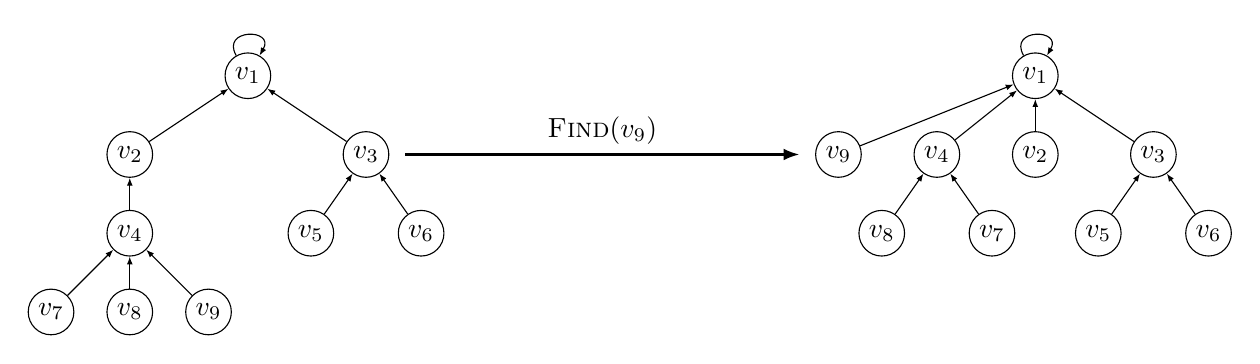
\begin{tikzpicture}[vertex/.style={circle, draw, fill=white, inner sep=2pt}]
		\begin{scope}
			\node[vertex] (1) at (0, 0) {$v_1$};
			\node[vertex] (22) at (1.5, -1) {$v_3$};
			\node[vertex] (21) at (-1.5, -1) {$v_2$};
			\node[vertex] (31) at (-1.5, -2) {$v_4$};
			\node[vertex] (32) at (0.8, -2) {$v_5$};
			\node[vertex] (33) at (2.2, -2) {$v_6$};
			\node[vertex] (41) at (-0.5, -3) {$v_9$};
			\node[vertex] (42) at (-1.5, -3) {$v_8$};
			\node[vertex] (43) at (-2.5, -3) {$v_7$};
			\path (1) edge [out=120, in=60, loop, min distance=0.4cm, -{Latex[length=1mm]}] (1);
			\draw[-{Latex[length=1mm]}] (21) -- (1);
			\draw[-{Latex[length=1mm]}] (22) -- (1);
			\draw[-{Latex[length=1mm]}] (31) -- (21);
			\draw[-{Latex[length=1mm]}] (32) -- (22);
			\draw[-{Latex[length=1mm]}] (33) -- (22);
			\draw[-{Latex[length=1mm]}] (41) -- (31);
			\draw[-{Latex[length=1mm]}] (42) -- (31);
			\draw[-{Latex[length=1mm]}] (43) -- (31);
		\end{scope}
		\begin{scope}[shift={(10,0)}]
			\node[vertex] (A1) at (0, 0) {$v_1$};
			\node[vertex] (A22) at (1.5, -1) {$v_3$};
			\node[vertex] (A21) at (0, -1) {$v_2$};
			\node[vertex] (A31) at (-1.25, -1) {$v_4$};
			\node[vertex] (A32) at (0.8, -2) {$v_5$};
			\node[vertex] (A33) at (2.2, -2) {$v_6$};
			\node[vertex] (A41) at (-0.55, -2) {$v_7$};
			\node[vertex] (A42) at (-1.95, -2) {$v_8$};
			\node[vertex] (A43) at (-2.5, -1) {$v_9$};
			\path (A1) edge [out=120, in=60, loop, min distance=0.4cm, -{Latex[length=1mm]}] (A1);
			\draw[-{Latex[length=1mm]}] (A21) -- (A1);
			\draw[-{Latex[length=1mm]}] (A22) -- (A1);
			\draw[-{Latex[length=1mm]}] (A31) -- (A1);
			\draw[-{Latex[length=1mm]}] (A32) -- (A22);
			\draw[-{Latex[length=1mm]}] (A33) -- (A22);
			\draw[-{Latex[length=1mm]}] (A41) -- (A31);
			\draw[-{Latex[length=1mm]}] (A42) -- (A31);
			\draw[-{Latex[length=1mm]}] (A43) -- (A1);
		\end{scope}
		\draw[thick, -{Latex[length=2mm]}, shorten <=2mm, shorten >= 2mm] (22) -- node[midway, above] {\textsc{Find}$(v_9)$} (A43);
	\end{tikzpicture}
	\captionof{figure}{Path compression during \textsc{Find}$(v_9)$ operation}
\end{center}
Here is the pseudocode of the \textsc{Find} operation below:
\begin{algorithm}[]
	\caption{\textsc{Find}$(v)$}
	\DontPrintSemicolon
	\If{$v.\emph{parent}\neq v$}{
		$v.\emph{parent}\longleftarrow \textsc{Find}(v.\emph{parent})$\;
	}
	\Return{$v.\emph{parent}$}
\end{algorithm}We will not discuss the amortized cost of this operation. Instead, we will do it in \autoref{analysis-union-find}.
\subsection{\textsc{Union} Operation}
For the \textsc{Union} operation we change the root of smaller rank to point to the root of the component of larger rank. So for the \textsc{Union}$(u,v)$ operation we assume that $u$, $v$ are the roots of their respective components. 
\begin{algorithm}[]
	\caption{\textsc{Union}$(u,v)$}
	\SetKwComment{Comment}{// }{}
	\DontPrintSemicolon
	\If{$u.\emph{rank}>v.\emph{rank}$}{
		$v.\emph{parent}\longleftarrow v$\;
	}
	\ElseIf{$v.\emph{rank}>u.\emph{rank}$}{
		$u.\emph{parent}\longleftarrow v$\;
	}
	\Else{
		$v.\emph{parent}\longleftarrow u$\;
		$v.\emph{rank}\longleftarrow v.\emph{rank}+1$
	}
\end{algorithm}
Since in \textsc{Union}$(u,v)$ we assume $u,v$ are component representatives before using \textsc{Union}$(u,v)$ we use \textsc{Find} on $u$ and $v$ to get the roots of their components, and then we apply \textsc{Union} on the roots. Hence, \textsc{Union}$(u,v)$ takes $O(1)$ time.
\subsection{Analyzing the Union-Find Data-Structure}\label{analysis-union-find}
We call a node in the union-find data-structure a \emph{leader} if it is the root of the (reversed) tree.
\begin{lemma}{}{}
	Once a node stop being a {leader} (i.e. the node in top of a tree). It can never become a leader again.
\end{lemma}
\begin{proof}
	A node $x$ stops being a {leader} only because of the \prb{Union} operation which made $x$ child of a node $y$ which is a {leader} of a tree. From this point on, the only operation that might change the parent pointer of $x$ is the \prb{Find} operation which traverses through $x$. Since path-compression only change the parent pointer of $x$ to point to some other node $y$. Therefore, the parent pointer of $x$ will never become equal to itself i.e. $x$ can never be a {leader} again. Hence, once $x$ stops being a {leader} it can never be a {leader} again.
\end{proof}
\begin{lemma}{}{}
	Once a node stop being a leader then its rank is fixed.
\end{lemma}
\begin{proof}
	The rank of a node changes only by a \prb{Union} operation. But the \prb{Union} operation only changes the rank of nodes that are {leader} after the operation is done. Therefore, once a node stops being a {leader} it's rank will not being changed by a \prb{Union} operation. Hence, once a node stop being a leader then its rank is fixed.
\end{proof}
\begin{lemma}{}{}
	Ranks are monotonically increasing in the reversed trees, as we travel from a node to
	the root of the tree.
\end{lemma}
\begin{proof}
	To show that the ranks are monotonically increasing  it suffices to prove that for all edge $u\to v$ in the data structure we have $\Rank(u)<\Rank(v)$.
\end{proof}

\begin{lemma}{}{}
	When a node gets rank $k$ than there are at least $\geq 2^k$ elements in its subtree.
\end{lemma}
\begin{corolary}{}{}
	For all vertices $v$, $v.rank\leq \lt\lfloor \log n\rt\rfloor$
\end{corolary}
\begin{corolary}{}{}
	Height of any tree $\leq \lt\lfloor\log _2n\rt\rfloor$
\end{corolary}
\begin{lemma}{}{}
	The number of nodes that get assigned rank $k$ throughout the execution of the Union-Find data-structure is at most $\frac{n}{2^k}$.
\end{lemma}
Define $N(r)=\#$vertices with rank at least $k$. Then by the above lemma we have $N(r)\leq \frac{n}{2^k}$.
\begin{lemma}{}{}
	The time to perform a single find operation when we perform union by rank and path
	compression is $O(\log n)$ time.
\end{lemma}
We will show that we can do much better. In fact, we will show that for $m$ operations over $n$ elements the overall running time is $O((n+m)\log ^*n)$

\begin{lemma}{}{}
	During a single $\prb{Find}(x)$ operation, the number of jumps between blocks along the search path is $O(\log^*n)$.
\end{lemma}
\begin{lemma}{}{}
	At most $|\emph{Block}(i)|\leq \emph{Tower}(i)$ many \prb{Find} operations can pass through an element $x$ which is in the $i^{th}$ block (i.e. $\prb{index}_B(x)=i$) before $x.\emph{parent}$ is no longer in the $i^{th}$ block. That is $\prb{index}_B(x.\emph{parent})>i$.
\end{lemma}

\begin{lemma}{}{}
	There are at most $\frac{n}{\emph{Tower}(i)}$ nodes that have ranks in the $i^{th}$ block throughout the algorithm execution.
\end{lemma}

\begin{lemma}{}{}
	The number of internal jumps performed, inside the $i^{th}$ block, during the lifetime of \prb{Union-Find} data structure is $O(n)$.
\end{lemma}

\begin{Theorem}{}{}
	The number of internal jumps performed by the \prb{Union-Find} data structure overall $O(n\log^*n)$.
\end{Theorem}
\begin{Theorem}{}{}
	The overall time spent on $m$ \prb{Find} operations, throughout the lifetime of a Union-Find data structure defined over $n$ elements is $O((n+m)\log^*n)$.
\end{Theorem}